% Final report (M4), CCU Operating Systems, Fall 2026.
% Build: cd paper_ieee && latexmk -pdf main.tex   (or: pdflatex main; bibtex main; pdflatex main; pdflatex main)
\documentclass[conference]{IEEEtran}
\IEEEoverridecommandlockouts

\usepackage[utf8]{inputenc}
\usepackage[T1]{fontenc}
\usepackage{lmodern}
\usepackage{amsmath}
\usepackage{graphicx}
\usepackage{booktabs}
\usepackage{siunitx}
\usepackage{xcolor}
\usepackage{url}
\usepackage[hidelinks]{hyperref}
\usepackage{cite}

\graphicspath{{../results/phase6b/}{../results/phase5d/}}
\sisetup{detect-all, group-minimum-digits=4}

\newcommand{\Lrel}{L_{\mathrm{rel}}}
\newcommand{\us}{\,\textmu s}

\begin{document}

\title{Where Should a 10\,ms Control Loop Live?\\
Benchmarking Linux and Zephyr on a Heterogeneous Edge Controller}

\author{
\IEEEauthorblockN{Quang-Huy Nguyen}
\IEEEauthorblockA{Student ID 615461004\\
Dept.\ of International Master Program\\
in Smart Manufacturing\\
National Chung Cheng University, Taiwan}
\and
\IEEEauthorblockN{An-Rui Peng}
\IEEEauthorblockA{Student ID 614461008\\
Dept.\ of International Master Program\\
in Smart Manufacturing\\
National Chung Cheng University, Taiwan}
}

\maketitle

\begin{abstract}
Prescriptive maintenance asks one edge controller to run heavy analytics and, at the same time, act on a machine within a hard deadline. We study where such a 10\,ms control loop should run on the Arduino UNO Q, a board that pairs a quad-core Linux processor with a Zephyr microcontroller. We compare four configurations under identical work: a Linux thread under the default fair scheduler (A), the same thread under \texttt{SCHED\_FIFO} with locked memory (B), B on a core reserved by affinity (B-iso), and the loop on the microcontroller with setpoints sent from Linux (C). Loads range from \texttt{stress-ng} to realistic edge work: bulk Wi-Fi traffic and a containerised CNN fed by a vibration stream. One lateness definition is applied to every configuration. Under the heaviest realistic load, the typical worst case per 10{,}000 cycles was 5.6\,ms for A, 0.31\,ms for B, 1.46\,ms for B-iso and 9\us{} for C; every Linux configuration missed the 1\,ms deadline (3.5\,\%, 0.025\,\% and 0.23\,\% of cycles), while C missed none in 20{,}000 cycles and delivered all 1{,}920 speed commands to an emulated drive. Two results explain the gap. \texttt{SCHED\_FIFO} preempts programs but not the kernel's interrupt and softirq work, which is why reserving a core made B worse. On the microcontroller, thread priority decided the outcome: with library defaults the communication thread delayed the loop by up to 0.8\,ms, and raising the loop above it reduced this about 100-fold. We report 95\,\% intervals for all headline figures.
\end{abstract}

\begin{IEEEkeywords}
real-time systems, Linux scheduling, SCHED\_FIFO, Zephyr RTOS, asymmetric multiprocessing, edge computing, prescriptive maintenance
\end{IEEEkeywords}

\section{Introduction}
\label{sec:intro}

Industrial maintenance is moving from \emph{predictive} to \emph{prescriptive}. A predictive system analyses vibration and reports a likely fault to a person, so a late result costs seconds. A prescriptive system acts on its own: it lowers spindle speed or changes the feed when the analysis says so. That closes a control loop, and the loop has a hard deadline.

Consider a CNC cell with a sensory tool holder. Vibration is streamed to an AI model on a Linux ``digital twin'' host, which also handles program downloads, camera uploads and plant networking. A 10\,ms loop applies the resulting speed or feed override. The AI's advice may arrive many milliseconds late without harm, because tool wear develops over minutes. The loop that changes the machine's command may not be late.

This exposes an operating-system dilemma. A general-purpose OS such as Linux offers the software stack the analytics need, but its scheduler and the kernel's own work can delay a time-critical thread. A real-time OS such as Zephyr bounds timing by design but cannot run the analytics stack. Asymmetric multiprocessing (AMP) boards put both on one board: the Arduino UNO Q~\cite{arduino_unoq} pairs a Qualcomm QRB2210 (four Cortex-A53 cores, Debian Linux) with an STM32U585 microcontroller (Cortex-M33, Zephyr).

We ask: \emph{where should the 10\,ms loop run so that a busy Linux side cannot make it late?} Our contributions are:
\begin{itemize}
\item A like-for-like comparison of four placements of the same loop (A, B, B-iso, C; Section~\ref{sec:system}) on real hardware, with one lateness definition for all of them and an external timing referee.
\item Measurements under both synthetic load (\texttt{stress-ng}) and realistic edge load (Wi-Fi traffic and a containerised CNN), including the full chain from analytics to an emulated motor drive.
\item Two explanations of the results: kernel work, not CPU load, limits \texttt{SCHED\_FIFO} on a stock kernel; and thread priority, not the RTOS itself, decides the microcontroller's timing.
\item Uncertainty for every headline figure (intervals on miss ratios, bootstrap ranges on worst cases and ratios), so the size of each claim is clear.
\end{itemize}

Section~\ref{sec:background} reviews the scheduling background, Section~\ref{sec:system} describes the system, Section~\ref{sec:method} the method, Section~\ref{sec:results} the results and Section~\ref{sec:discussion} their interpretation. Section~\ref{sec:limitations} states the limitations and Section~\ref{sec:conclusion} concludes.

\section{Background}
\label{sec:background}

\subsection{Scheduling on Linux}
Ordinary Linux threads use \texttt{SCHED\_OTHER}, served by the fair scheduler. Since kernel 6.6 this is EEVDF (earliest eligible virtual deadline first~\cite{stoica1995eevdf,linux_sched_eevdf}), which replaced CFS. A fair scheduler shares the CPU in proportion to weight, so a time-critical thread waits behind every other runnable thread for its turn.

The real-time policies \texttt{SCHED\_FIFO} and \texttt{SCHED\_RR} (priorities 1--99) always run ahead of \texttt{SCHED\_OTHER}: a woken \texttt{SCHED\_FIFO} thread preempts a normal program at once~\cite{linux_sched_rt}. Locking memory with \texttt{mlockall} removes page faults from its path. What a real-time thread cannot preempt is the kernel's own work in interrupt context: hardware interrupt handlers, inter-processor interrupts (IPIs) and the softirq processing (network receive, timers, RCU) that runs when an interrupt returns. A stock kernel built with \texttt{PREEMPT} also keeps sections that cannot be preempted. The \texttt{PREEMPT\_RT} patch set moves most of this work into schedulable threads and makes most kernel sections preemptible~\cite{reghenzani2019rtlinux}; our board runs the stock \texttt{PREEMPT} kernel.

Placement matters as well. Affinity can pin a thread to one core and steer movable interrupts away from it, but without boot-time isolation (\texttt{isolcpus}, \texttt{nohz\_full}) the kernel can still schedule its own work on that core.

\subsection{Scheduling on Zephyr}
Zephyr is a priority-based, preemptive RTOS. Every thread has a fixed priority, and a lower number means a higher priority; a ready thread of higher priority preempts a lower one immediately~\cite{zephyr_threads}. Timing on an RTOS is therefore only as good as its priority assignment: a library thread placed above the control loop delays the loop whenever it runs.

\subsection{Prescriptive maintenance workload}
Our analytics use the Case Western Reserve University (CWRU) bearing data~\cite{cwru_data,smith2015cwru}: 12\,kHz vibration from healthy bearings and from bearings with inner-race, ball and outer-race faults. A 1{,}024-sample window spans 85.3\,ms, which sets the analytics cadence. A Hann window and FFT give the peak frequency, which a simple rule maps to a speed setpoint (100, 85, 70 or 60\,\%).

% Owner: Quang-Huy Nguyen (P7.1: hardware setup, Linux experiments, IPC implementation). Draft by An-Rui Peng; please review.
\section{System Design}
\label{sec:system}

\subsection{Hardware}
The device under test (DUT) is an Arduino UNO Q~\cite{arduino_unoq}: a Qualcomm QRB2210 with four Cortex-A53 cores at up to 2.016\,GHz, running Debian~13 with the stock kernel 6.16 (\texttt{PREEMPT}, not \texttt{PREEMPT\_RT}), and an STM32U585 Cortex-M33 at 160\,MHz running the Zephyr-based Arduino core. The two chips communicate over Arduino's RouterBridge, a remote-procedure-call layer over an internal serial link. Two further UNO Q boards complete the bench (Fig.~\ref{fig:bench}): a \emph{referee} timestamps the DUT's tick pulse on pin D2 with its own DWT cycle counter, and a \emph{drive emulator} decodes the speed command that the DUT sends as 500\,Hz PWM on pin D3. A PC starts every run over USB and generates the network load over Wi-Fi.

\begin{figure}[t]
\centering
\setlength{\fboxsep}{6pt}
\fbox{\parbox{0.92\columnwidth}{\small
\textbf{PC} --- Wi-Fi (traffic, sensor stream) $\rightarrow$ \textbf{DUT}\\[2pt]
\textbf{DUT, Linux side:} load, analytics, loop in A/B/B-iso\\
\textbf{DUT, MCU side:} loop in C\\[2pt]
DUT D2 (tick pulse) $\rightarrow$ \textbf{Referee} (times every tick)\\
DUT D3 (500\,Hz PWM speed command) $\rightarrow$ \textbf{Drive emulator}\\
PC --- USB/adb (control only) --- all boards; grounds joined}}
\caption{Test bench: DUT, external referee and drive emulator.}
\label{fig:bench}
\end{figure}

\subsection{The control loop and the analytics}
Every configuration runs the same minimal loop: wake at the next release time of a fixed 10\,ms schedule, read the latest setpoint, store a timestamp in RAM, and sleep. Nothing is written to storage during a run. The analytics (Hann window, 1{,}024-point FFT, setpoint rule) run separately every 85.33\,ms on replayed CWRU frames, so only the operating system's behaviour differs between configurations.

On Linux the loop is a thread of a C benchmark that sleeps with \texttt{clock\_nanosleep(CLOCK\_MONOTONIC, TIMER\_ABSTIME)}; the analytics run in a second, normal-priority thread. On the MCU the loop is an Arduino sketch scheduled with \texttt{micros()}: it records the DWT cycle counter, reads the setpoint, emits a 500\us{} pulse on D2, sleeps 6\,ms when more than 3\,ms remain, and spins to the release time.

\subsection{Configurations}
\begin{itemize}
\item \textbf{A}: the Linux loop thread under \texttt{SCHED\_OTHER} (EEVDF).
\item \textbf{B}: the same thread under \texttt{SCHED\_FIFO}, priority 90, with \texttt{mlockall}.
\item \textbf{B-iso}: B pinned to core 3; our load, the analytics and the 51 movable interrupts (of 81) moved to cores 0--2; deep CPU idle states disabled through \texttt{/dev/cpu\_dma\_latency}. Isolation is by affinity only, with no boot-time isolation.
\item \textbf{C}: the loop on the MCU. Linux sends each new setpoint over RouterBridge; in the full-chain runs the MCU also outputs it as PWM to the drive emulator.
\end{itemize}

\subsection{Linux-to-MCU link}
The link is ``latest value wins''. Linux calls \texttt{set\_setpoint(seq, sp)}; the MCU handler packs the sequence number and setpoint into one aligned 32-bit word, \texttt{(seq $\ll$ 8) | sp}, which is a single atomic store on the Cortex-M33. The loop reads that word once per tick with one load and logs it, so it never waits for Linux and never sees a torn value. A late message delays the advice, never the tick.

On Zephyr a lower number means a higher priority. With the Arduino library defaults (\emph{stock}) the sketch's loop runs at priority 14 and RouterBridge's bridge thread at 5, so message handling can preempt the loop. The \emph{tuned} variant raises the loop to priority 4 with one call at the end of \texttt{setup()}; everything else is unchanged. We report both.

\section{Measurement Method}
\label{sec:method}

\subsection{Lateness}
Cycle $k$ has release time $R_k = t_0 + 10k$\,ms and wake time $t_k$. We report lateness relative to the run's best cycle,
\begin{equation}
\Lrel(k) = (t_k - R_k) - \min_j (t_j - R_j),
\end{equation}
for every configuration. On Linux, $t_k$ comes from \texttt{CLOCK\_MONOTONIC}. On the MCU, $t_k$ comes from the DWT cycle counter; Zephyr's timekeeping loses cycles while the MCU sleeps, so the loop's true period is about 10.0055\,ms, and we fit the period by least squares before computing lateness. Removing this constant offset leaves jitter and worst cases unchanged. A cycle with $\Lrel > 1$\,ms is a deadline miss.

The referee independently timestamps every tick pulse with its own DWT counter. An earlier referee used Zephyr's \texttt{k\_cycle\_get\_32()}, which loses cycles while sleeping; it reported an apparent $-390$\,ppm offset between the boards that disappeared ($-0.3$ to $+3$\,ppm) once the referee used DWT. Its largest deviation then matched the DUT's own worst case in the same runs.

\subsection{Loads}
\textbf{Synthetic.} \texttt{stress-ng}~\cite{stressng} in four tiers: idle; \emph{core-0 medium} (one CPU worker on core 0, one disk and one memory worker using 25\,\% of RAM); \emph{core-0 heavy} (two CPU and two cache workers on core 0, disk, memory at 50\,\%); and \emph{all-core} (four CPU workers and the same cache, disk and memory workers; three CPU workers on cores 0--2 for B-iso).

\textbf{Realistic.} \texttt{rnet}: the PC sends bulk TCP over Wi-Fi, which the board receives at 5.8--6.8\,MB/s and discards. \texttt{rdeploy}: the PC streams CWRU vibration at its real rate (about 48\,kB/s) to a Docker container running a 1D-CNN under ONNX Runtime with three threads, at 11.7 inferences per second. \texttt{rboth}: both at once. Before, during and after each run the board checked that the load was present; all 60 checks passed.

\subsection{Protocol}
Linux runs are 180{,}000 cycles (30\,min); MCU runs are 10{,}000 cycles (100\,s), the most timestamps the MCU can hold. Linux runs used the \texttt{performance} governor at a fixed 2.016\,GHz; Config C runs kept the board default (\texttt{schedutil}), which does not affect the MCU's timing. No run reached thermal throttling (maximum 64.8\,\textdegree C). Synthetic tiers have 3 runs per Linux condition and 3--4 per Config C condition (1--2 for all-core); realistic tiers have 2 runs each. We wrote 15 predictions down before the realistic and full-chain runs and report which held.

\subsection{Statistics}
A longer run catches a larger worst case, so we split every run into 10{,}000-cycle blocks and compare the median of the block worst cases (``block WCL''). For miss ratios we give 95\,\% Wilson intervals~\cite{wilson1927}; with zero misses in $n$ cycles we give the exact one-sided 95\,\% bound $1-0.05^{1/n} \approx 3/n$. Block medians get 95\,\% bootstrap intervals~\cite{efron1993bootstrap} over pooled blocks. Config C has one block per run, so ratio ranges divide the Linux interval by C's worst and best block. Blocks within a run are correlated, so these intervals are optimistic; where two runs disagree beyond their intervals we quote the per-run values.

\section{Results}
\label{sec:results}

\subsection{Synthetic load}
Table~\ref{tab:synthetic} summarises the \texttt{stress-ng} tiers. Default Linux (A) missed deadlines in every loaded tier, up to 39.2\,\% of cycles under core-0 heavy load, and its worst case reached 18.0--27.9\,ms under all-core load. \texttt{SCHED\_FIFO} (B) held the deadline in every tier, although one run reached 973\us{}. B-iso stayed near 0.3\,ms under any stress. Config C with tuned priorities stayed at about 8\us{} at every tier, idle included: Linux load did not reach it.

\begin{table}[t]
\centering
\caption{Worst-case lateness under \texttt{stress-ng} (µs, mean of runs; DMR = highest miss ratio of any run)}
\label{tab:synthetic}
\small
\setlength{\tabcolsep}{3.5pt}
\resizebox{\columnwidth}{!}{%
\begin{tabular}{@{}lrrrrr@{}}
\toprule
Config & Idle & Core-0 med. & Core-0 heavy & All-core & DMR \\
\midrule
A & 545 & 5{,}304 & 6{,}321 & 21{,}580 & 39.2\,\% \\
B & 471 & 755 & 489 & 661 & 0 \\
B-iso & 96 & 324 & 329 & 324 & 0 \\
C, IPC stock & 759 & 795 & 809 & 759 & 0 \\
C, IPC tuned & 8.1 & 7.9 & 7.7 & 7.8 & 0 \\
\bottomrule
\end{tabular}}
\\[2pt]\footnotesize Source: \texttt{results/phase5d/compare\_configs.md}; 3 runs per cell (C all-core: 1).
\end{table}

\texttt{stress-ng} only creates busy programs, which a real-time thread preempts at once. The realistic loads below also make the kernel work.

\subsection{Realistic load}
Table~\ref{tab:realload} gives the worst cases and miss ratios under realistic load, and Fig.~\ref{fig:blocks} shows the worst case of every 10{,}000-cycle block. A's blocks sat at 4--15\,ms whenever the CNN ran. B stayed below 1\,ms under the CNN alone (\texttt{rdeploy}: 0 misses in 360{,}000 cycles) but crossed it once network traffic was added. B-iso exceeded 1\,ms in all 36 of its \texttt{rboth} blocks. Config C stayed between 6.3 and 10.5\us{} in every tier, idle included, with no misses.

\begin{table}[t]
\centering
\caption{Realistic load: worst case (range of 2 runs), typical block worst case, and misses over 1\,ms with 95\,\% interval}
\label{tab:realload}
\small
\setlength{\tabcolsep}{2.5pt}
\resizebox{\columnwidth}{!}{%
\begin{tabular}{@{}llrrl@{}}
\toprule
Config & Tier & WCL (ms) & Block (ms) & Misses (\%) \\
\midrule
A & rnet & 1.49--1.71 & 0.56 & 0.0022 (0.0011--0.0044) \\
A & rdeploy & 11.8--15.0 & 5.89 & 1.48 (1.45--1.52) \\
A & rboth & 8.36--10.7 & 5.61 & 3.54; runs 4.72, 2.36 \\
B & rnet & 0.99--1.16 & 0.73 & 0.0011 (0.0004--0.0029) \\
B & rdeploy & 0.52--0.55 & 0.14 & 0 ($\le$0.0008) \\
B & rboth & 1.45--1.54 & 0.31 & 0.025 (0.020--0.031) \\
B-iso & rnet & 0.76--0.82 & 0.52 & 0 ($\le$0.0008) \\
B-iso & rdeploy & 0.57--0.65 & 0.40 & 0 ($\le$0.0008) \\
B-iso & rboth & 1.59--1.72 & 1.46 & 0.23 (0.22--0.25) \\
C & idle & 0.0063--0.0070 & 0.0067 & 0 ($\le$0.015) \\
C & rnet & 0.0081--0.0083 & 0.0082 & 0 ($\le$0.015) \\
C & rdeploy & 0.0070--0.0082 & 0.0076 & 0 ($\le$0.015) \\
C & rboth & 0.0076--0.0105 & 0.0091 & 0 ($\le$0.015) \\
\bottomrule
\end{tabular}}
\\[2pt]\footnotesize Linux: 2 runs $\times$ 180{,}000 cycles; C: 2 runs $\times$ 10{,}000 cycles. Sources: \texttt{results/phase6b/realload.md}, \texttt{headline\_stats.md}.
\end{table}

\begin{figure}[t]
\centering
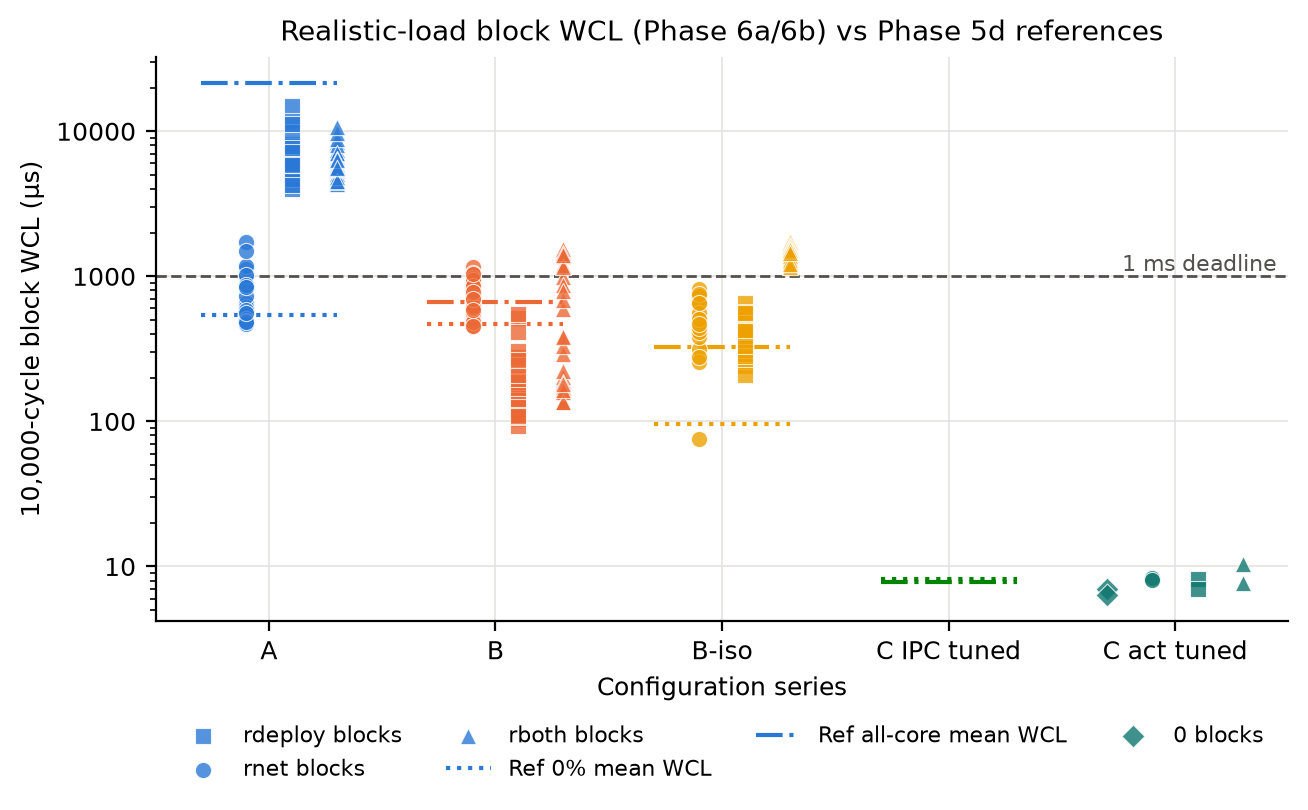
\includegraphics[width=\columnwidth]{block_wcl.png}
\caption{Worst-case lateness of every 10{,}000-cycle block under realistic load (log scale; dashed line: 1\,ms deadline). Config C stays near 10\us{} in every tier.}
\label{fig:blocks}
\end{figure}

Compared per block under \texttt{rboth}, Config C's typical worst case was 34$\times$ below B (plausible range 18--103$\times$, because B's blocks vary widely), 161$\times$ below B-iso (133--197$\times$) and 619$\times$ below A (528--797$\times$). The gap to B was smallest under the CNN alone, 19$\times$ (16--24$\times$), and largest under network traffic alone, 88$\times$ (82--98$\times$).

\subsection{Reserving a core made SCHED\_FIFO worse}
Under \texttt{rboth}, B-iso's worst case (1.59--1.72\,ms) and miss ratio (0.23\,\%) were worse than plain B's (1.45--1.54\,ms, 0.025\,\%). Fig.~\ref{fig:cpu3} shows the kernel work counted on core 3. Under \texttt{rboth} the ``reserved'' core received 654 function-call IPIs per second in B-iso against 60 in B, and about 440 against 220 softirqs per second. It was 24\,\% busy although none of our programs ran there; under the CNN alone it was only 4\,\% busy. Under \texttt{rnet} alone core 3 received \emph{less} kernel work in B-iso than in B, yet B-iso still exceeded the 0.5\,ms we predicted, so another mechanism, such as shared cache or memory traffic, may contribute.

\begin{figure}[t]
\centering
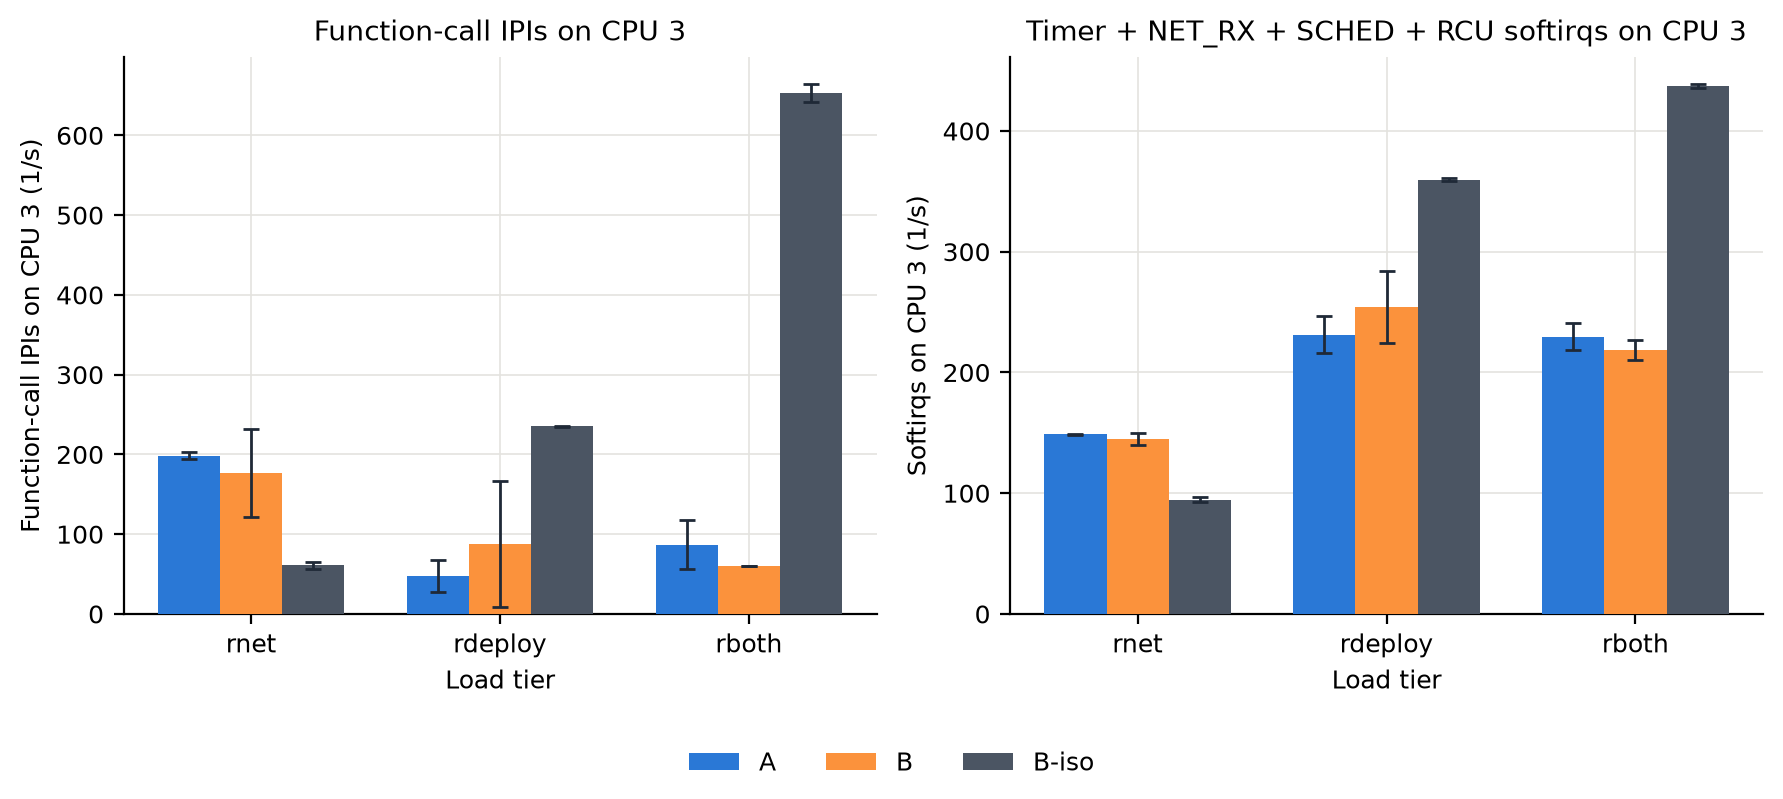
\includegraphics[width=\columnwidth]{cpu3_kernel_work.png}
\caption{Kernel work per second on CPU 3 for B and B-iso (run averages over 2 repeats).}
\label{fig:cpu3}
\end{figure}

\subsection{On the microcontroller, priority decided the result}
Table~\ref{tab:mcu} compares the four Config C variants under \texttt{stress-ng}. With library defaults, adding the link raised the worst case from 20--41\us{} to 759--809\us{}, already at idle. In the stock IPC runs, 72--83\,\% of the late cycles (over 100\us) contained a setpoint arrival, against a base rate of 11.7\,\%. Raising the loop above the bridge thread brought the IPC worst case to 7.7--8.1\us{} and the number of such late cycles from 84--121 per run to zero. The tuned link still costs about 6\us{} over the tuned baseline.

\begin{table}[t]
\centering
\caption{Config C variants under \texttt{stress-ng}: worst case (µs), range of tier means}
\label{tab:mcu}
\small
\begin{tabular}{@{}lll@{}}
\toprule
Variant & Loop priority & Worst case \\
\midrule
Stock, no IPC & below bridge (14 vs 5) & 20--41 \\
Stock, with IPC & below bridge & 759--809 \\
Tuned, no IPC & above bridge (4 vs 5) & 1.5--1.7 \\
Tuned, with IPC & above bridge & 7.7--8.1 \\
\bottomrule
\end{tabular}
\\[2pt]\footnotesize 3--4 runs per tier. Source: \texttt{results/phase5d/compare\_configs.md}, \texttt{ipc\_attribution.md}.
\end{table}

\subsection{The full chain to the drive}
In eight Config C runs (idle and the three realistic tiers, two each), all 1{,}920 speed commands reached the drive emulator with the right value: none lost, wrong or duplicated. The drive saw each new command 1.47--4.11\,ms after the tick that applied it, and this delay was the same at idle and under every load, because it is set by the 500\,Hz PWM (waiting for the next period plus the pulse width), not by Linux. Linux load only stretched the time a setpoint took to reach the MCU: the 99th-percentile round trip grew from 12.8\,ms at idle to 15.7\,ms under \texttt{rboth}. The loop never waited for it.

\subsection{Predictions}
Of the 15 predictions written before the realistic and full-chain runs, 12 held, one held partly and two failed. A's miss ratio under \texttt{rdeploy} exceeded the predicted 1\,\% (1.42--1.55\,\%). B-iso under \texttt{rnet} stayed above 0.5\,ms although the Wi-Fi interrupt had been moved off core 3. The setpoint round trip under \texttt{rnet} was not longer than at idle: the sender suffers from CPU contention, not from network interrupts.

\section{Discussion}
\label{sec:discussion}

\subsection{What limits each configuration}
\textbf{A} competes with the CNN's threads for CPU time under a fair scheduler and waits several milliseconds for its turn; CPU-heavy work (\texttt{rdeploy}) hurts it most.

\textbf{B} preempts every normal program at once, which is why it kept every \texttt{rdeploy} cycle under 1\,ms with two cores near 100\,\% busy. It cannot preempt interrupt handlers or the softirq work that runs when an interrupt returns, and network traffic produces exactly that work. This is the most likely reason network traffic pushed B past 1\,ms; we did not trace it.

\textbf{B-iso} illustrates the same limit more sharply. Moving our programs and the movable interrupts away left core 3 as the only core with spare time, and the kernel placed more of its own work there. Under \texttt{rboth} the whole board was equally busy in B and B-iso (about 71\,\%), and B's loop shared cores that were 40--85\,\% busy, yet B's worst case beat B-iso's on a core only 24\,\% busy. For a real-time thread on a stock kernel, the non-preemptible kernel work on its core matters more than how busy the core looks. The counters are run averages: they are consistent with this explanation but do not prove the cause of each late cycle.

\textbf{C} runs on a separate processor with its own RTOS. Linux load could delay the setpoint, never the tick, and the tick's worst case changed by only a few microseconds between idle and the heaviest load. The one large effect on C came from inside the MCU: with library defaults, the communication thread outranked the control loop. An RTOS does not make a loop real-time by itself; its priority assignment does.

\subsection{What this means for the CNC example}
Assume a feed of 6\,m/min (100\,mm/s). A tick that runs late leaves the machine on its previous command for that long. A's worst delay (10.7\,ms) is about 1.1\,mm of tool travel on the old command, and at its measured miss ratios it would be late 8{,}500--17{,}000 times per hour. B's worst delay (1.54\,ms) is 0.15\,mm, late 50--130 times per hour. Config C's worst delay (10.5\us) is about 1\,µm. No rate can be extrapolated from zero misses in 20{,}000 cycles, but its worst case is 100$\times$ below the deadline. The design that follows matches how such cells are built in industry: let the digital-twin host be as busy as it needs, since its advice arriving 16\,ms late is harmless for wear that develops over minutes, and run the loop that acts on the machine on a dedicated real-time processor.

\section{Limitations}
\label{sec:limitations}

\textbf{The CNN was not trained.} The analytics node runs a 1D-CNN with random weights, sized so one inference takes about 40\,ms on the board. It is realistic background load, not a fault classifier, so the setpoints sent to the MCU come from the FFT rule, not from the CNN. This does not affect the timing study, but we make no claim about fault-detection accuracy.

\textbf{The MCU loop does not use a Zephyr timer.} Our plan specified a periodic Zephyr \texttt{k\_timer}. All MCU results use the Arduino sketch's \texttt{micros()} schedule with a 6\,ms sleep and a final spin. A \texttt{k\_timer} version was never run on the board. The loop also has a latent flaw found in code review: if a cycle ever started more than about 3.5\,ms late, its 6\,ms sleep would overshoot the next release. This never happened (C's worst case was about 10\us), and the measured code was left unchanged.

\textbf{Several explanations are untested.} (i) Earlier single runs showed Linux slower at idle than under load (median 224\us{} for A and 171\us{} for B at idle, 44\us{} for B under load). We attribute this to waking from deep CPU idle states. It is consistent with B-iso, which disables them, having a 5$\times$ smaller idle worst case than B (96 vs 471\us), but B-iso also changes pinning and interrupt placement, so the effect is not isolated. (ii) In an early test, locking memory with \texttt{mlockall} under memory pressure gave \emph{higher} lateness than not locking it (mean 413 vs 208\us); this was not explained, and we do not cite it as evidence for or against \texttt{mlockall}. (iii) The kernel work on B-iso's core is consistent with its higher lateness but was not traced per cycle; a kernel trace would settle it.

\textbf{No \texttt{PREEMPT\_RT} kernel.} B and B-iso ran on the stock \texttt{PREEMPT} kernel. \texttt{PREEMPT\_RT} moves most interrupt and softirq work into schedulable threads~\cite{reghenzani2019rtlinux} and would likely narrow the gap between B and C; our Linux results are therefore not the best real-time Linux can do.

\textbf{Scope of the evidence.} One board set; an emulated drive instead of a motor; two repeats per realistic condition, the two \texttt{rboth} repeats in one session. MCU runs are 18$\times$ shorter than Linux runs, which is why we compare per block and why C's zero misses bound its miss ratio only at 0.015\,\%. The CNN runtime lets idle worker threads spin by default~\cite{onnxruntime_threads}; we kept the default, as a typical deployment would, so the CNN tiers occupy more CPU than inference needs.

\section{Conclusion}
\label{sec:conclusion}

We placed the same 10\,ms control loop in four places on one heterogeneous edge controller and measured it under synthetic and realistic load with one lateness definition. Four findings stand out.

First, \texttt{SCHED\_FIFO} makes Linux robust against busy programs but not against the kernel's own work. Under network traffic plus a containerised CNN, every Linux configuration missed the 1\,ms deadline, the best of them in 0.025\,\% of cycles with a worst case of 1.5\,ms.

Second, reserving a core by affinity alone made \texttt{SCHED\_FIFO} worse, not better, because the kernel moved its interrupt and softirq work onto the reserved core.

Third, the real-time microcontroller kept every tick within about 10\us{} at every load level, a typical worst case 34$\times$ below the best Linux configuration (range 18--103$\times$) and about 600$\times$ below default Linux, and delivered all 1{,}920 speed commands to the emulated drive. Linux load delayed only the setpoint, which the loop never waits for.

Fourth, the microcontroller's advantage depended on one priority setting. With library defaults its communication thread delayed the loop by up to 0.8\,ms; raising the loop above it reduced the cost about 100-fold.

For prescriptive maintenance on AMP hardware, the answer to our question is: run the analytics on Linux and the loop that acts on the machine on the real-time core, with the loop given the highest priority there. Priorities are part of the design on both sides.

\section*{Individual Contributions}
\textbf{Quang-Huy Nguyen} built and ran everything on the boards: the Linux benchmark and harness, the Config C sketches and link, the referee and drive-emulator apps, the realistic-load setup, all measurement runs and clock diagnostics, and the comparison scripts for Phases 5 and 6.

\textbf{An-Rui Peng} defined the measurement method with Huy, wrote the latency analysis pipeline and the statistical analysis (error bars, block comparison), reviewed the Phase 2 and Phase 5--6 code and results, and drafted the progress reports, the presentation and this report.

\section*{Reproducibility}
All raw data (\texttt{results/raw/}), analysis scripts with tests (\texttt{benchmarks/analysis/}), board apps and the harness are in the project repository. Every table cites the result file it was taken from.


\bibliographystyle{IEEEtran}
\bibliography{references}

\end{document}
